\documentclass[12pt,a4paper]{article}
% Course format: A4, 12-pt Times New Roman, 2.5 cm margins, single spacing.
\usepackage[a4paper,margin=2.5cm]{geometry}
\usepackage[T1]{fontenc}
\usepackage{mathptmx}   % Times New Roman text and math
\usepackage{graphicx}
\usepackage{booktabs}
\usepackage{amssymb}
\usepackage{tabularx}
\usepackage{multirow}
\usepackage{algorithm}
\usepackage{algpseudocode}
\usepackage{amsmath}
\usepackage{xcolor}
\usepackage[hidelinks]{hyperref}
\usepackage{caption}
\usepackage{enumitem}
\usepackage{titlesec}

\graphicspath{{../iot_agent/results/figures/}{../presentation/}}
\captionsetup{font=small,labelfont=bf,skip=4pt}
\setlist{nosep,leftmargin=*}
\titlespacing*{\section}{0pt}{8pt}{3pt}
\titlespacing*{\subsection}{0pt}{6pt}{2pt}
\setlength{\parskip}{2pt}
\setlength{\textfloatsep}{8pt}
\setlength{\floatsep}{6pt}
\setlength{\intextsep}{6pt}
\newcommand{\code}[1]{\texttt{\small #1}}
\renewcommand{\arraystretch}{1.05}

\begin{document}

%-------------------------------------------------------------- cover page
\begin{titlepage}
\centering
\vspace*{4cm}
{\Large The Hong Kong Polytechnic University\par}
\vspace{0.6cm}
{\large COMP5511 Artificial Intelligence Concepts --- Final Project Report\par}
\vspace{2.2cm}
{\LARGE\bfseries AI Agent for Smart Security IoT Systems\par}
\vspace{2.2cm}
{\large Student name: Zhang Chi\par}
\vspace{0.3cm}
{\large Student ID: 25064822g\par}
\vfill
{\large November 2026\par}
\end{titlepage}

%-------------------------------------------------------------- 1
\section{Motivation}
In consumer smart security systems built around a central gateway, cameras and sensors cannot reach the
network on their own: pairing, data transport, video streaming, firmware synchronisation and cloud reporting all
pass through one base station. During an internship at an IoT security company I worked on frontline support
tickets for such a system together with field application engineers (FAEs). Most tickets were not caused by
broken hardware but by \emph{interaction faults} between the base station and its peripherals: pairing timeouts,
weak links, protocol mismatches after firmware updates, blocked cloud uplinks or inconsistent binding tables.

Frontline staff had no standard troubleshooting procedure, so escalation depended on personal experience. Two
costs followed. Simple, self-recoverable faults were escalated and consumed scarce FAE time, while genuinely
complex faults (protocol conflicts, simultaneous loss of several devices) were buried among them and resolved late.
The task is therefore not only \emph{diagnosis} but \emph{triage}: decide whether a ticket can be closed at frontline
(tier L1, with repair steps and a reply template) or must go to an FAE (tier L2, with a complete escalation ticket).

This is a natural agentic problem. As in web agents that observe an environment, plan and act on
feedback~\cite{webagents}, the evidence here is spread over a support console, a knowledge base and facts that only
the customer can observe, so a useful assistant must plan which evidence to collect, call tools, ask questions,
react to the results and stop at the right time. The intended users are frontline support staff; the agent is a
copilot that suggests questions and actions to the staff member, who relays them to the customer. FAEs benefit
from fewer and better-structured tickets. This is an \textbf{application project}; its contributions are
(i) a topology-ordered evidence planner and typed session memory for this master--slave domain, (ii) a
policy-derived rule layer that can only raise the tier, (iii) a labelled benchmark of 52 support cases with a
separate challenge set, and (iv) an evaluation against four baselines and four ablations with significance tests
and repeated runs.

%-------------------------------------------------------------- 2
\section{Description of the Approach}

Figure~\ref{fig:arch} shows the workflow. Its design follows how an experienced engineer works on a master--slave
system: check the master first, then the binding table, then the links, the firmware and finally the peripheral
itself. The approach combines four components.

\begin{figure}[!ht]
\centering
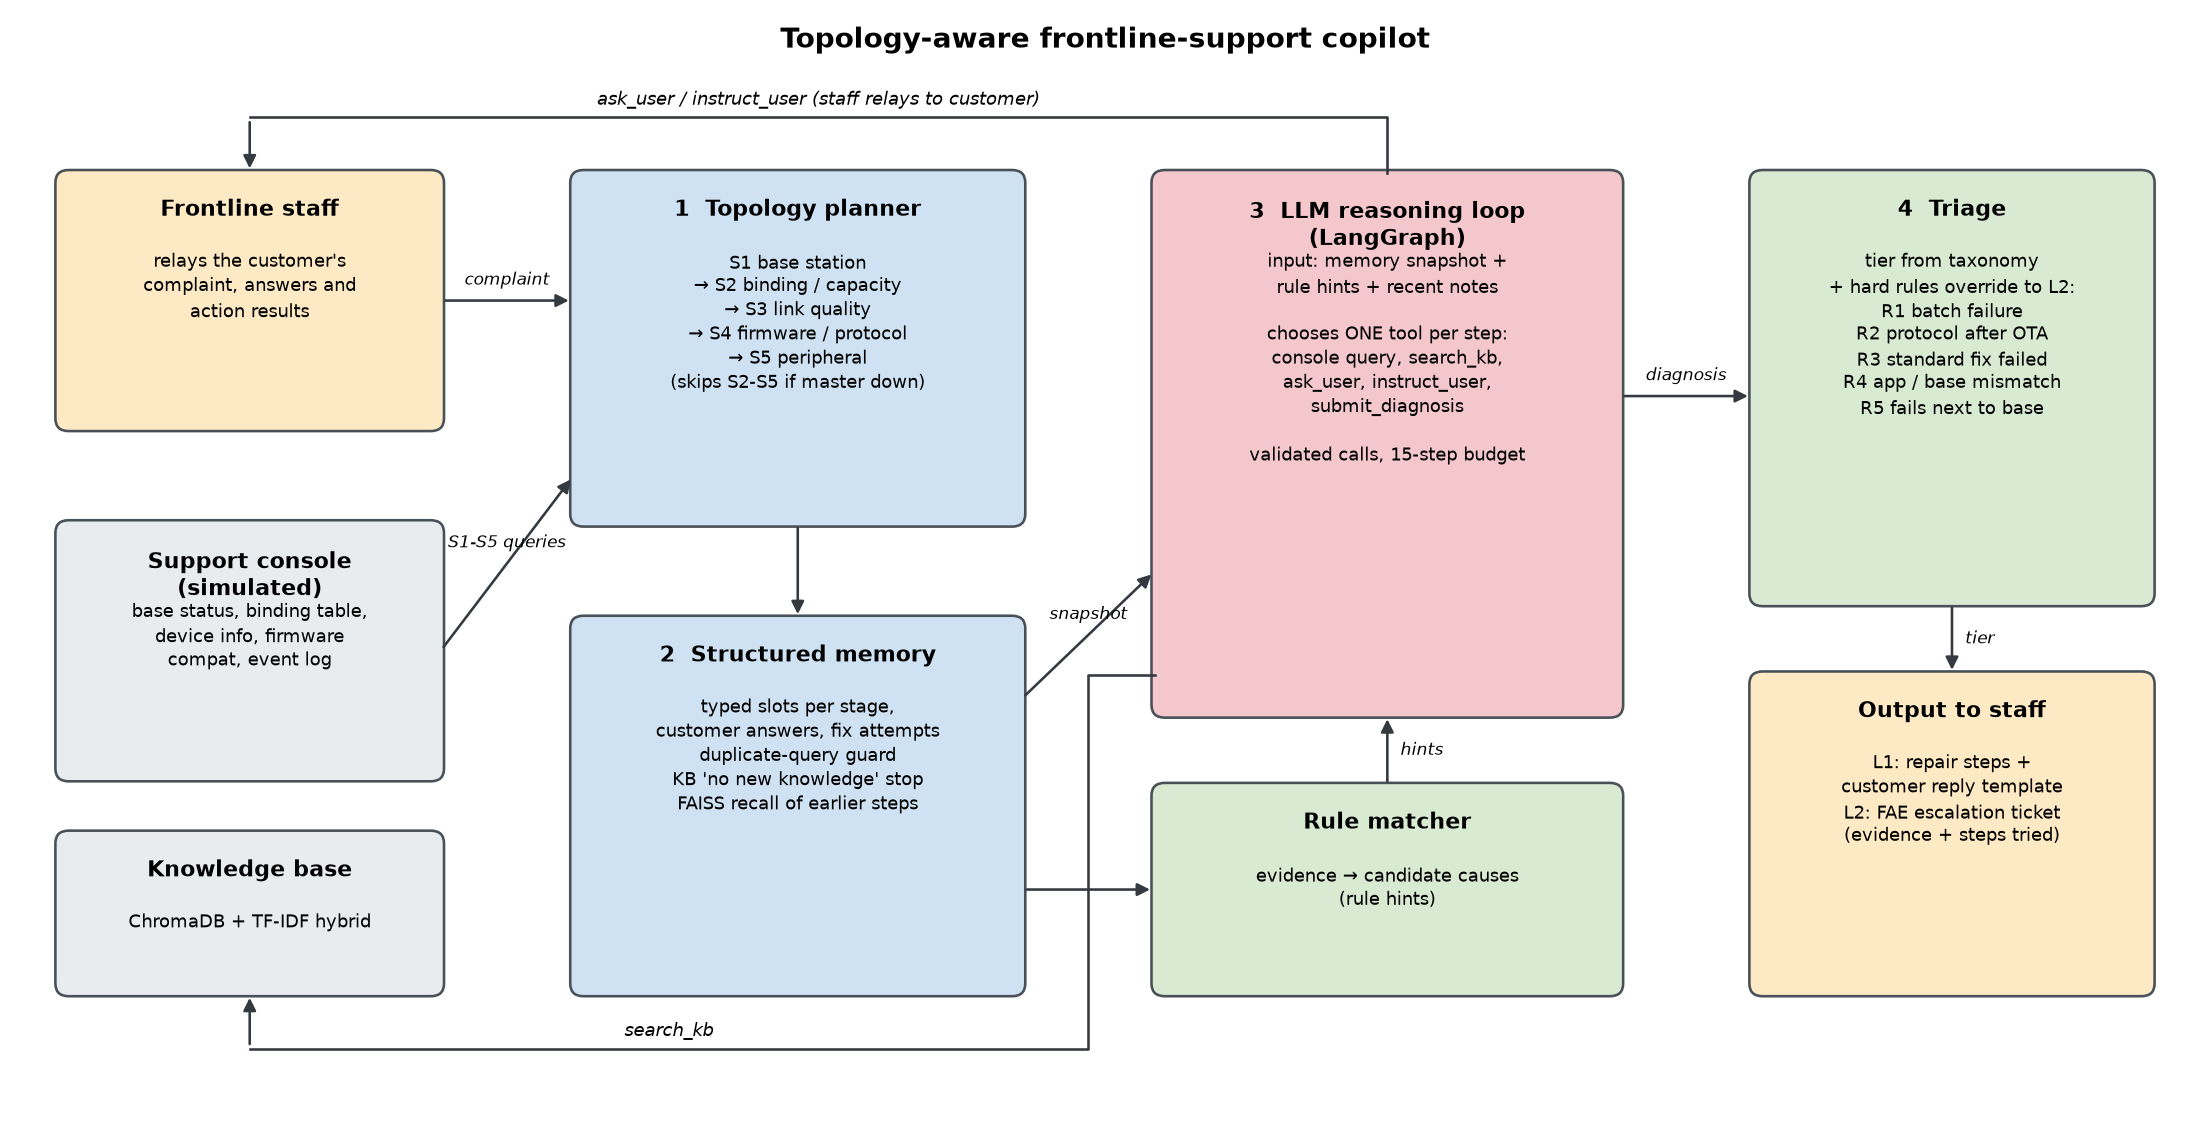
\includegraphics[width=\linewidth]{architecture.png}
\caption{Architecture of the topology-aware copilot. Deterministic components (blue, green) collect and check
evidence; the LLM (red) chooses one tool per step. Staff relay \code{ask\_user}/\code{instruct\_user} to the customer.}
\label{fig:arch}
\end{figure}

\textbf{(1) Topology planner.} Before any LLM call, the planner queries the support console in the fixed order
S1 base station $\rightarrow$ S2 binding/capacity $\rightarrow$ S3 link quality $\rightarrow$ S4
firmware/protocol $\rightarrow$ S5 peripheral. It prunes queries that the hierarchy makes uninformative: if the
base station is offline every peripheral only mirrors that failure, so S2--S5 are skipped; otherwise only devices
that are abnormal in the binding table (at most five) are inspected. This front-loads cheap, deterministic evidence.

\textbf{(2) Structured session memory.} Confirmed facts are stored in typed slots (base status, binding table,
per-device info, compatibility, logs, KB snippets, customer answers, fix attempts) instead of a raw transcript.
The slots drive the planner's bookkeeping, the rule matcher and two guards: a duplicate-query guard answers any
console query or customer question that was already answered, and a knowledge-search guard returns a ``no new
knowledge'' note when a KB search only yields snippets already in memory and refuses further searches after two
such searches in a row. A FAISS index over earlier steps provides short recall of the session.

\textbf{(3) LLM reasoning loop.} At each step the LLM receives the complaint, the memory snapshot, the rule hints
and its recent notes, and calls exactly one tool: a console query, \code{search\_kb}, \code{ask\_user} (a question
the staff member should ask), \code{instruct\_user} (an action to walk the customer through, tagged with the cause it
is meant to fix) or \code{submit\_diagnosis} with one of 12 root-cause labels. Tool calls and results are validated
and the loop has a 15-step budget. After a guided action, a separate LLM call judges from the customer's reply
whether it resolved the problem (yes / no / unclear) and whether it was the standard fix for the targeted cause.

\textbf{(4) Rule-based triage.} The tier is first taken from the taxonomy entry of the diagnosed cause. Five hard
rules derived from the written escalation policy can then only \emph{raise} it to L2:
R1 two or more bound peripherals failed at the same time while the base is online (E-610, or loss events within
5 minutes); R2 a protocol mismatch persists after a failed OTA or has no OTA path; R3 the standard fix for the
diagnosed L1 cause was performed and failed; R4 the app's device list and the base binding table disagree;
R5 the customer reports that the device still fails next to the base after a reset. A deterministic rule matcher
also turns confirmed evidence into candidate causes (rule hints) for the LLM. Finally the output writer produces
repair steps and a reply template (L1) or an escalation ticket with symptoms, devices, codes, steps tried and the
suspected cause (L2). Algorithms~\ref{alg:diag} and~\ref{alg:tier} summarise the procedure.

\textbf{Why this suits the task.} The domain has strong structure that a general ReAct agent must rediscover in
every session: a dependency order between components, a closed label set and an explicit escalation policy.
Encoding the order in a planner saves LLM steps; typed memory keeps the prompt focused and avoids repeated
questions; and rules make every escalation traceable to a policy clause, which matters when FAE time is the
scarce resource. The LLM is kept for what rules cannot do: interpreting free-text complaints and customer replies,
deciding what to ask, and reconciling conflicting evidence (for example a stale console reading).

\begin{algorithm}[t]
\caption{Topology-aware diagnosis}\label{alg:diag}
\small
\begin{algorithmic}[1]
\Require complaint $c$, console $E$, knowledge base $K$, step budget $B=15$
\Ensure root cause $y$, tier $t\in\{\mathrm{L1},\mathrm{L2}\}$, hand-off document $o$
\State $M \gets \textsc{Memory}(c)$
\While{$q \gets \textsc{NextQuery}(M)$ exists} \Comment{S1$\to$S2$\to$S3$\to$S4$\to$S5, pruned}
  \State $M.\textsc{Update}(q, E(q))$
\EndWhile
\For{$i = 1$ \textbf{to} $B$}
  \State $H \gets \textsc{MatchCauses}(M)$; \ $a \gets \textsc{LLM}(c, M.\textsc{Snapshot}(), H, \text{notes})$
  \If{$a = \textsc{Submit}(y)$} \textbf{break} \EndIf
  \If{$a$ was already answered} $r \gets M.\textsc{Lookup}(a)$ \Comment{duplicate-query guard}
  \ElsIf{$a = \textsc{SearchKB}$ and $M.\mathit{stale} \ge 2$} $r \gets$ ``KB exhausted, decide now''
  \ElsIf{$a = \textsc{SearchKB}$} $r \gets K(a)$; $M.\mathit{stale} \gets$ ($r$ has a new snippet) ? $0$ : $M.\mathit{stale}+1$
  \ElsIf{$a = \textsc{Instruct}(\mathit{act}, \mathit{cause})$}
    \State $r \gets$ customer reply; \ $M.\textsc{AddAction}(\mathit{act},\mathit{cause},\textsc{Judge}(r))$
  \Else\ $r \gets \textsc{Execute}(a)$
  \EndIf
  \State $M.\textsc{Update}(a, r)$
\EndFor
\If{no diagnosis was submitted} $y \gets$ first cause in $H$ \EndIf
\State $(t, R) \gets \textsc{ClassifyTier}(M, y)$; \ $o \gets$ repair steps if $t=\mathrm{L1}$, else FAE ticket
\State \Return $y, t, o$
\end{algorithmic}
\end{algorithm}

\begin{algorithm}[t]
\caption{\textsc{ClassifyTier}: taxonomy tier with policy override}\label{alg:tier}
\small
\begin{algorithmic}[1]
\Require memory $M$, diagnosed cause $y$
\State $t \gets \mathrm{taxonomy}[y].\mathit{tier}$; \ $R \gets \emptyset$
\If{$\ge 2$ bound devices lost within 300\,s (or E-610) and base online} $R \gets R \cup \{\mathrm{R1}\}$ \EndIf
\If{protocol mismatch and (OTA failed or no OTA path)} $R \gets R \cup \{\mathrm{R2}\}$ \EndIf
\If{$t=\mathrm{L1}$ and the standard fix for $y$ was performed and failed} $R \gets R \cup \{\mathrm{R3}\}$ \EndIf
\If{app device list $\ne$ base binding table} $R \gets R \cup \{\mathrm{R4}\}$ \EndIf
\If{customer: reset $\wedge$ device next to base $\wedge$ still failing} $R \gets R \cup \{\mathrm{R5}\}$ \EndIf
\If{$R \ne \emptyset$} $t \gets \mathrm{L2}$ \Comment{rules can only escalate}\EndIf
\State \Return $t, R$
\end{algorithmic}
\end{algorithm}

%-------------------------------------------------------------- 3
\section{Implementation}
The system is written in Python. External components are DeepSeek chat models~\cite{deepseek} through the
OpenAI-compatible SDK (\code{deepseek-v4-pro} for the agent, \code{deepseek-flash} for the simulated customer and the
judges, thinking mode disabled, temperature 0), LangGraph~\cite{langgraph} for orchestration and checkpointing,
ChromaDB~\cite{chroma} with the \code{BAAI/bge-small-en-v1.5} embedding model~\cite{bge} and a TF-IDF ranking fused by
reciprocal rank fusion~\cite{rrf} for knowledge retrieval, FAISS~\cite{faiss} for in-session recall, and Streamlit for
a staff dashboard. The proposal planned the openJiuwen platform~\cite{openjiuwen}; I used LangGraph instead because it
runs locally and its SQLite checkpointer directly supports pausing the graph while a staff member relays a customer
reply. All other code (planner, memory, rules, workflow, environment, cases, baselines and evaluation) is my own.
Table~\ref{tab:code} lists the key functions and variables.

\begin{table}[t]
\centering\small
\caption{Key modules, functions and variables of the implementation (\code{iot\_agent/}).}\label{tab:code}
\footnotesize\renewcommand{\code}[1]{\texttt{#1}}
\begin{tabularx}{\linewidth}{@{}lX@{}}
\toprule
File & Key functions / variables \\
\midrule
\code{agent/planner.py} & \code{next\_query(memory)}: next console query in S1$\to$S5 order; \code{master\_down()}; \code{MAX\_DEVICES\_INSPECTED}=5 \\
\code{agent/memory.py} & \code{SessionMemory}: typed slots, \code{lookup()} duplicate guard, \code{update()}, \code{add\_action()}, \code{snapshot()}, \code{stale\_kb\_searches} \\
\code{agent/workflow.py} & \code{build\_workflow()}: LangGraph nodes \code{collect}, \code{reason}, \code{tool}, \code{validate}, \code{wait}, \code{finish}; \code{judge\_action\_reply()} \\
\code{agent/agent.py} & \code{TopologyAgent.run(env)}; \code{\_search\_kb()} with \code{KB\_STALE\_LIMIT}=2; \code{ABLATIONS} \\
\code{agent/rules.py} & \code{match\_causes()} (rule hints), \code{escalation\_triggers()} (R1--R5); thresholds \code{WEAK\_RSSI}=$-80$\,dBm, \code{LOW\_BATTERY}=10\,\%, \code{SIMULTANEOUS\_WINDOW\_S}=300 \\
\code{agent/triage.py} & \code{classify\_tier()} (Algorithm~\ref{alg:tier}), \code{build\_output()} (repair steps or FAE ticket) \\
\code{env/case\_env.py} & \code{CaseEnv}: console tools \code{get\_base\_status}, \code{get\_topology}, \code{get\_device\_info}, \code{check\_firmware\_compat}, \code{get\_logs}; \code{ask\_user}, \code{instruct\_user} \\
\code{env/user\_simulator.py} & \code{UserSimulator}: LLM customer restricted to the facts of the case \\
\code{eval/} & \code{baselines.py}, \code{run\_cases.py} (\code{--run N} for repeats), \code{metrics.py}, \code{stats.py} (Wilson, McNemar), \code{report.py} \\
\bottomrule
\end{tabularx}
\end{table}

\textbf{Environment.} Real tickets cannot be shared, so each case is a simulated support session. \code{CaseEnv}
exposes the console tools over the case's hidden state (base station, devices, logs) and a product catalogue
(base-station capacity, firmware protocols, OTA paths). The customer is played by an LLM that may only use the
facts and scripted action outcomes listed in the case, sees only what the phone app would show, and must never
name the root cause. Every system that interacts with the customer therefore faces the same information limits.

\textbf{Knowledge base.} Five fictional documents (base-station manual, peripheral manual, fault-code reference,
escalation policy and seven historical cases) are split into 30 chunks, one per section. Hybrid search reached
top-3 hits on 13/13 retrieval probes (dense retrieval alone missed 2 of the original 12).

\textbf{Engineering.} All model calls go through one function with retries, token accounting and an on-disk cache
keyed by the full request, so re-running an experiment is fast and reproducible; repeated runs use a separate
cache namespace so the model is really called again. The code has 78 unit tests that run without an API key (the
LLM is mocked), including a worst-case test that feeds every scripted customer fact of every case into memory and
checks that R5 never fires on an L1 case.

%-------------------------------------------------------------- 4
\section{Data}
I built a labelled benchmark of 52 cases (Table~\ref{tab:data}) because no public dataset covers gateway-centric
security systems with frontline/FAE labels. Each case contains a customer complaint, the hidden console state, facts
only the customer knows, scripted outcomes of customer actions, and the ground-truth root cause (one of 12 labels),
tier and key troubleshooting stages. Five cases were written by hand from internship experience; C006--C040 are
produced by a deterministic generator from scenario templates. To make the cases realistic and resistant to
keyword matching, every case carries distractors: a multi-sentence complaint that often contains a wrong
self-diagnosis (blaming batteries, the router or the app), a household of 5--9 devices including healthy devices
with borderline signal or battery, 4--12 log lines with routine noise, and several ineffective customer actions
besides the real fix. Distractors never change the label evidence.

\begin{table}[t]
\centering\small
\caption{Case statistics. The challenge set is always reported separately.}\label{tab:data}
\begin{tabular}{@{}lcc@{}}
\toprule
Statistic & Core (C001--C040) & Challenge (C041--C052) \\
\midrule
Cases / root-cause labels & 40 / 12 & 12 / 11 \\
L1 (frontline) / L2 (FAE) & 24 / 16 & 6 / 6 \\
Easy / medium / hard & 5 / 22 / 13 & 0 / 0 / 12 \\
Devices / log lines per case (mean) & 6.7 / 8.2 & 6.3 / 5.5 \\
Complaint length (words, mean) & 58.8 & 49.3 \\
Customer facts / action outcomes (mean) & 4.5 / 3.6 & 3.3 / 3.6 \\
\bottomrule
\end{tabular}
\end{table}

A first evaluation showed that the core set can largely be solved by shortcuts: rules alone reached 92\% and an LLM
that reads only the complaint 85\%. I therefore wrote a \textbf{challenge set} (C041--C052) in which each case
defeats one shortcut. In three cases the console shows a stale reading that only the customer can correct (for
example a camera whose last RSSI was recorded at its old location); in the other nine the decisive evidence is on
the console but the complaint points confidently to the wrong cause. The labels are balanced over 12 causes in the
core set (2--4 cases each), and the tier split (60\% L1) mirrors the motivation that most tickets should be closed
at frontline. Because the cases, the knowledge base and the policy are synthetic and written by me, the benchmark is
suitable for controlled comparisons between systems but is not an independent estimate of real-world accuracy
(Section~\ref{sec:disc}).

%-------------------------------------------------------------- 5
\section{Experiment Setting, Baselines and Performance}
\textbf{Systems.} Each baseline isolates part of the design. \emph{Vanilla LLM} sees only the complaint and answers in
one call. \emph{Vanilla RAG} additionally receives the three best KB snippets. \emph{Rules only} runs the planner and
the rule matcher with no LLM (taking the strongest rule hint, then Algorithm~\ref{alg:tier}). \emph{ReAct}~\cite{react}
is a standard reason--act loop with exactly the same tools, budget and action judge as our agent but without the
planner, rule hints, typed memory and rule override; it reasons over the raw transcript. Four ablations remove one
component of our agent each.

\textbf{Metrics.} Root-cause accuracy; tier accuracy; escalation precision (share of L2 decisions that needed an FAE)
and recall (share of real L2 cases escalated); customer interaction rounds; LLM calls, tokens and model seconds per
case; and a 1--5 usability score from an LLM judge~\cite{llmjudge} that sees the complaint, the output and the
record of questions asked and actions performed. Because the sets are small, I report 95\% Wilson
intervals~\cite{wilson} and exact two-sided McNemar tests~\cite{mcnemar} on the paired per-case outcomes, and I
repeated the two tool-using agents three times.

\begin{table}[t]
\centering\small
\caption{Main results. Run 1 for all systems; italic rows: mean $\pm$ s.d.\ of root-cause and tier accuracy over three runs of the two tool-using agents. Rounds: questions and actions relayed to the customer per case. Usab.: LLM judge, 1--5.}\label{tab:main}
\setlength{\tabcolsep}{4pt}
\resizebox{\linewidth}{!}{\begin{tabular}{@{}llcccccccc@{}}
\toprule
Set & System & Cause acc & Tier acc & L2 prec. & L2 rec. & Rounds & Usab. & Tokens & Sec. \\
\midrule
\multirow{7}{*}{Core} & Vanilla LLM & 85\% & 88\% & 87\% & 81\% & 0.00 & 3.27 & 884 & 6.5 \\
 & Vanilla RAG & 85\% & 88\% & 82\% & 88\% & 0.00 & 3.45 & 1257 & 6.3 \\
 & Rules only & 92\% & 92\% & 100\% & 81\% & 0.00 & 2.05 & 0 & 0.0 \\
 & ReAct (same tools) & 92\% & 98\% & 94\% & 100\% & 0.72 & 3.05 & 14946 & 19.2 \\
 & \textbf{Topology (ours)} & \textbf{100\%} & \textbf{100\%} & \textbf{100\%} & \textbf{100\%} & 1.12 & \textbf{3.92} & 17181 & 21.6 \\
 & \emph{ReAct, 3 runs} & \emph{94.2$\pm$1.4} & \emph{96.7$\pm$1.4} & & & & & & \\
 & \emph{Topology, 3 runs} & \emph{100.0$\pm$0.0} & \emph{99.2$\pm$1.4} & & & & & & \\
\midrule
\multirow{7}{*}{Chall.} & Vanilla LLM & 25\% & 50\% & 50\% & 17\% & 0.00 & 3.42 & 876 & 6.2 \\
 & Vanilla RAG & 33\% & 58\% & 67\% & 33\% & 0.00 & 3.50 & 1228 & 6.7 \\
 & Rules only & 75\% & 75\% & 100\% & 50\% & 0.00 & 1.92 & 0 & 0.0 \\
 & ReAct (same tools) & 92\% & 92\% & 100\% & 83\% & 0.50 & 3.08 & 12573 & 17.1 \\
 & \textbf{Topology (ours)} & \textbf{100\%} & \textbf{100\%} & \textbf{100\%} & \textbf{100\%} & 1.08 & \textbf{3.75} & 24513 & 27.5 \\
 & \emph{ReAct, 3 runs} & \emph{91.7$\pm$0.0} & \emph{91.7$\pm$0.0} & & & & & & \\
 & \emph{Topology, 3 runs} & \emph{97.2$\pm$4.8} & \emph{100.0$\pm$0.0} & & & & & & \\
\bottomrule
\end{tabular}}
\end{table}

\textbf{Overall accuracy is not the right lens.} Averaged over three runs the topology agent reaches 100.0\%
$\pm$ 0.0 root-cause and 99.2\% $\pm$ 1.4 tier accuracy on the core set and 97.2\% $\pm$ 4.8 / 100.0\% $\pm$ 0.0 on the
challenge set (Table~\ref{tab:main}); ReAct reaches 94.2\% $\pm$ 1.4 / 96.7\% $\pm$ 1.4 and 91.7\% / 91.7\%. These
numbers say little on their own: the rules-only baseline, with no LLM at all, already answers \textbf{46 of the 52
cases} (37/40 core, 9/12 challenge), and with so few cases even a perfect run has 95\% Wilson intervals of
[91\%, 100\%] ($n=40$) and [76\%, 100\%] ($n=12$). Exact McNemar tests confirm only the advantage over the
complaint-only baselines ($p\le0.031$ on both sets); the single-run gaps to rules only and ReAct (3 of 40 core cases)
are not significant ($p=0.25$). The question that matters for an LLM agent is therefore narrower: \emph{does the LLM
solve the cases the rules cannot, and does it stay reliable on the cases the rules already solve?}

\textbf{Hard cases: where the LLM is irreplaceable.} I define the \emph{rule-hard} subset as the six cases the
rules-only baseline gets wrong (three core, three challenge; pooled because they are too few to split). Rules only
scores 0\% there by construction; every system with an LLM solves at least four of them (Table~\ref{tab:hard}). The
six cases fall into two kinds. In four (C033--C035, C052) the customer states in the complaint that the standard
fixes were already tried; the rules cannot read this, while every LLM, even one that sees only the complaint, can.
In the other two (C041, C050) the console reading is stale and the complaint is misleading, so only an agent that
asks the customer can succeed: the complaint-only LLMs fail both, ReAct is right in 3 of 6 runs and our agent in 5 of
6 (C050: ReAct 0/3, ours 2/3). Over three runs our agent reaches 94.4\% root-cause and 100\% tier accuracy on the
rule-hard subset, against 83.3\% / 83.3\% for ReAct.

\textbf{Stability: where the structure is irreplaceable.} The pure tool-use loop pays for its flexibility on the easy
cases. On the 46 rule-easy cases ReAct is correct in all three runs on only 41 (pass$^3$ = 89\%) and changed its root
cause between runs on five, whereas our agent is correct on all 46 in every run (pass$^3$ = 100\%), because the
planner and the rule hints anchor it to the evidence. The planner also matters on the hard cases: without it the agent
solves only 3 of the 6 (single run). The two results are complementary: the LLM is needed where the console evidence
is insufficient, and the deterministic structure is needed to make the LLM reliable everywhere else.

\textbf{Example (C041).} The customer writes that the garage camera must have a weak signal and asks for a repeater; the
console shows $-83$\,dBm. Rules only and Vanilla LLM answer WEAK\_SIGNAL (L1). Our agent notices in the log that this
RSSI was recorded two days ago at the old location, asks the customer, learns that the LED stays dark after a reset and
after re-plugging the adapter, and escalates HW\_FAULT\_SUSPECTED (L2), which is correct.

\begin{table}[t]
\centering\small
\caption{Rule-easy vs rule-hard cases (rule-hard = the 6 cases the rules-only baseline gets wrong). For the two
tool-using agents: mean over 3 runs and pass$^3$ (correct in all 3 runs); other systems: one run. Bottom: correct
runs per rule-hard case.}\label{tab:hard}
\resizebox{\linewidth}{!}{\begin{tabular}{@{}lccccc@{}}
\toprule
& \multicolumn{2}{c}{Rule-easy (46 cases)} & \multicolumn{3}{c}{Rule-hard (6 cases)} \\
\cmidrule(lr){2-3}\cmidrule(lr){4-6}
System & Cause acc & pass$^k$ (cause) & Cause acc & Tier acc & pass$^k$ (cause / tier) \\
\midrule
Vanilla LLM & 71.7\% & 33/46 & 66.7\% & 66.7\% & 4/6 / 4/6 \\
Vanilla RAG & 73.9\% & 34/46 & 66.7\% & 66.7\% & 4/6 / 4/6 \\
Rules only (no LLM) & 100.0\% & 46/46 & 0.0\% & 0.0\% & 0/6 / 0/6 \\
ReAct (same tools), 3 runs & 94.9\% & 41/46 & 83.3\% & 83.3\% & 5/6 / 5/6 \\
\textbf{Topology (ours), 3 runs} & \textbf{100.0\%} & \textbf{46/46} & \textbf{94.4\%} & \textbf{100.0\%} & \textbf{5/6 / 6/6} \\
\bottomrule
\end{tabular}}

\vspace{4pt}
\resizebox{\linewidth}{!}{\begin{tabular}{@{}lcccccc@{}}
\toprule
& \multicolumn{4}{c}{Fixes already tried (complaint)} & \multicolumn{2}{c}{Stale console (dialogue needed)} \\
\cmidrule(lr){2-5}\cmidrule(lr){6-7}
System & C033 & C034 & C035 & C052 & C041 & C050 \\
\midrule
Vanilla LLM / Vanilla RAG & \checkmark & \checkmark & \checkmark & \checkmark & $\times$ & $\times$ \\
Rules only & $\times$ & $\times$ & $\times$ & $\times$ & $\times$ & $\times$ \\
ReAct (3 runs) & 3/3 & 3/3 & 3/3 & 3/3 & 3/3 & 0/3 \\
Topology (ours, 3 runs) & 3/3 & 3/3 & 3/3 & 3/3 & 3/3 & 2/3 \\
\bottomrule
\end{tabular}}
\end{table}

\textbf{Run-to-run errors.} Both of our agent's errors across the repeated runs involve rule R3. In C050 (run 2) the
agent did not ask whether the camera had been reset and diagnosed BATTERY\_LOW, but the failed charging attempt
triggered R3 and the tier stayed correct. In C008 (run 3) the
simulated customer improvised a base-station restart after being told to wait for the ISP, the action judge counted
it as a failed standard fix, and R3 caused one unneeded escalation.

\begin{table}[t]
\centering\small
\caption{Ablations (run 1). Repeats: identical console queries/questions per case blocked by memory / actually executed.}\label{tab:abl}
\setlength{\tabcolsep}{3.5pt}
\resizebox{\linewidth}{!}{\begin{tabular}{@{}lcccccc@{}}
\toprule
Variant & Core cause / tier & Unneeded / missed & LLM calls & Tokens & Repeats bl.\ / exec. & Chall.\ cause / tier \\
\midrule
Full agent & 100\% / 100\% & 0 / 0 & 6.5 & 17181 & 0.12 / 0.00 & 100\% / 100\% \\
$-$ topology planner & 98\% / 98\% & 0 / 1 & 10.2 & 28592 & 0.45 / 0.00 & 83\% / 100\% \\
$-$ rule hints & 98\% / 95\% & 2 / 0 & 7.2 & 20391 & 0.30 / 0.00 & 100\% / 100\% \\
$-$ structured memory & 100\% / 100\% & 0 / 0 & 7.2 & 18005 & 0.00 / 0.23 & 100\% / 100\% \\
$-$ rule tier override & 100\% / 100\% & 0 / 0 & 6.5 & 17181 & 0.12 / 0.00 & 100\% / 100\% \\
\bottomrule
\end{tabular}}
\end{table}

\textbf{Ablations.} Table~\ref{tab:abl} attributes the results to components. The \emph{planner} matters mostly for
cost: without it the LLM collects the console evidence itself, needing 57\% more LLM calls and 66\% more tokens, and
challenge accuracy drops to 83\%. The \emph{rule hints} prevent unneeded escalations (two on the core set without
them). Removing \emph{structured memory} does not lower accuracy on these cases; it only lets repeated queries reach
the console (0.23 per case), so its value here is efficiency and a cleaner prompt rather than accuracy. The
\emph{rule override} never fires in run 1, because the LLM's diagnosis already carries the right taxonomy tier; its
only visible effect is the rescued tier in C050 above. Ablation differences on the challenge set are one or two
cases and should not be over-interpreted.

\textbf{Cost.} Our agent uses about 15\% more tokens than ReAct on the core set (17.2k vs 14.9k per case, 6.5 LLM calls
each) and about twice as many on the challenge set (24.5k vs 12.6k). The cost breakdown shows why: it walks the
customer through more guided actions (0.67 vs 0.25 per case), searches the KB more (2.1 vs 1.0) and sends a larger
prompt per call (3.0k vs 2.2k tokens) because the memory snapshot is included at every step. With thinking mode
disabled a case takes about 20--30 seconds of model time.

\textbf{A failure we fixed.} In an earlier run our agent's only challenge error was C045, a ``ghost binding'': a sensor
deleted in the app still occupies the eighth slot of the base station, so pairing fails with a capacity error. The
KB had no procedure for this, the agent rephrased \code{search\_kb} 13 times until its budget ran out, and the
fallback took the first rule hint (CAPACITY\_EXCEEDED). Three changes fixed it: the knowledge-search guard, ordering
the more specific binding-mismatch hint before the capacity hint, and a KB section on orphaned bindings. C045 is now
solved with one search and 10k instead of 31k tokens, but it is no longer a held-out case.

%-------------------------------------------------------------- 6
\section{Discussion}\label{sec:disc}
\textbf{Why the approach works.} The hard-case analysis separates two jobs that a support agent must do. Reading
language and deciding what to ask is a job only the LLM can do: on the six cases the rules cannot solve, every LLM
system beats the rules, and only agents that talk to the customer solve the stale-console cases. Staying anchored to
the evidence is a job the deterministic structure does better: the planner and the rule hints keep our agent correct
in every run on the 46 easy cases, where a free tool-use loop drifts in 5 of them. Neither part is sufficient alone:
rules only fails every hard case, and ReAct is the least stable LLM system on easy ones. The rule layer adds
auditability on top: every L2 ticket cites the policy clause and evidence that triggered it.

\textbf{What the numbers do not show.} The high scores should be read with care. First, the labels, rules and
policy were written by the same person, so rule-based components are favoured by construction; this is why the
rules-only baseline already solves 46 of 52 cases (92\% of the core set) and why the override cannot be measured there (every core label's tier equals
its taxonomy tier). Second, the data is synthetic and the challenge set targets failure modes I already knew, so real
tickets, which are vaguer and noisier, would very likely give lower accuracy. Third, the usability scores come from
an LLM judge of the same model family; a blind 15-item human-rating sheet has been prepared to check agreement with
the judge but is not part of these results. Fourth, the simulated customer answers from a fixed fact list, while real
customers contradict themselves. Finally, the most fragile part of the system is the LLM action judge: R3 trusts its
verdict, and C008 shows that a single misjudged reply can cause an unneeded escalation.

\textbf{Possible improvements.} (i) Require R3 to see an explicit failed \emph{standard} action confirmed by the
staff member before escalating on R3 alone. (ii) Make the agent ask about resets and physical location whenever a
single device is offline with otherwise normal evidence, so R5 can apply (it fired only once and never changed an
outcome). (iii) Send only the memory slots that changed since the last step to cut the token cost of long sessions.
(iv) Evaluate on a small set of real, anonymised tickets and with human ratings.

\textbf{Insights.} Overall accuracy was the wrong lens for this project: on a benchmark where rules already solve
46 of 52 cases, every system looks good. Looking at the cases the rules cannot solve, and at whether a system is
correct in \emph{every} run, gave a clearer and more honest picture: the LLM is irreplaceable on the hard cases, and
deterministic domain structure is what makes it reliable on the rest. For agentic applications in narrow,
well-structured domains, this suggests evaluating on a rule-hard subset and with pass$^k$ rather than on average
accuracy, and building agents that let the structure handle the routine and the LLM handle the exceptions.

%-------------------------------------------------------------- references
\begingroup
\small
\begin{thebibliography}{99}
\setlength{\itemsep}{1pt}
\bibitem{webagents} L.~Ning, Z.~Liang, Z.~Jiang, et al. A survey of WebAgents: Towards next-generation AI agents for web automation with large foundation models. arXiv:2503.23350, 2025.
\bibitem{openjiuwen} openJiuwen Agent Platform. \url{https://openjiuwen.com/en/}.
\bibitem{react} S.~Yao, J.~Zhao, D.~Yu, N.~Du, I.~Shafran, K.~Narasimhan, Y.~Cao. ReAct: Synergizing reasoning and acting in language models. ICLR, 2023.
\bibitem{rrf} G.~V. Cormack, C.~L.~A. Clarke, S.~Buettcher. Reciprocal rank fusion outperforms Condorcet and individual rank learning methods. SIGIR, 2009.
\bibitem{bge} S.~Xiao, Z.~Liu, P.~Zhang, N.~Muennighoff. C-Pack: Packaged resources to advance general Chinese embedding. arXiv:2309.07597, 2023.
\bibitem{faiss} J.~Johnson, M.~Douze, H.~J\'egou. Billion-scale similarity search with GPUs. IEEE Transactions on Big Data, 7(3):535--547, 2019.
\bibitem{llmjudge} L.~Zheng, W.-L. Chiang, Y.~Sheng, et al. Judging LLM-as-a-judge with MT-Bench and Chatbot Arena. NeurIPS Datasets and Benchmarks, 2023.
\bibitem{wilson} E.~B. Wilson. Probable inference, the law of succession, and statistical inference. Journal of the American Statistical Association, 22(158):209--212, 1927.
\bibitem{mcnemar} Q.~McNemar. Note on the sampling error of the difference between correlated proportions or percentages. Psychometrika, 12(2):153--157, 1947.
\bibitem{langgraph} LangChain. LangGraph documentation. \url{https://langchain-ai.github.io/langgraph/}.
\bibitem{chroma} Chroma. ChromaDB documentation. \url{https://docs.trychroma.com/}.
\bibitem{deepseek} DeepSeek. DeepSeek API documentation. \url{https://api-docs.deepseek.com/}.
\end{thebibliography}
\endgroup

\end{document}
